\chapter{Transformations}
\section{Coordinates}
When trying to understand transformations it is a good idea to start off by looking at the coordinate system and that is what we will do here.  The system that we will use here describes the position of a point by saying how far it is across from an origin and how far up it is from an origin in that order.  We usually show this information as a pair of numbers in brackets seperated by a comma.

e.g. (5, 7)

which means 5 to the right and 7 up from the origin
\begin{center}
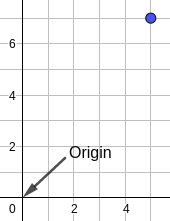
\includegraphics[scale=0.5]{./Images/Transformations/Basic_Coords.png}
\end{center}
We call the first number in the coordinate pair the $x$ coordinate and the second number the $y$ coordinate.

\begin{exmp}
Let's look at the diagram below and give the coordinates of the points.
\begin{center}
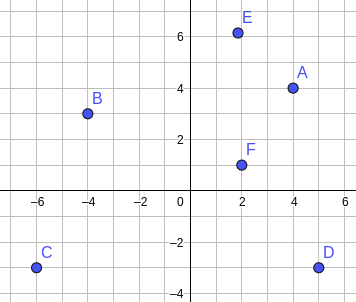
\includegraphics[scale=0.5]{./Images/Transformations/Coord_eg_1.png}
\end{center}
All the coordinates are done relative to the origin.

We can see that 'A' is 4 to the right and 4 up, so it's coordinates are $(4, 4)$

We can see that 'B' is 4 to the left and 3 up, so it's coordinates are $(-4, 3)$

We can see that 'C' is 6 to the left and 3 down, so it's coordinates are $(-6, -3)$

We can see that 'D' is 5 to the right and 3 down, so it's coordinates are $(5, -3)$

We can see that 'E' is 2 to the right and 6 up, so it's coordinates are $(2, 6)$

We can see that 'F' is 1 to the right and 1 up, so it's coordinates are $(2, 1)$
\end{exmp}
\subsection{Exercise}
Find the coordinates of the following points
\begin{center}
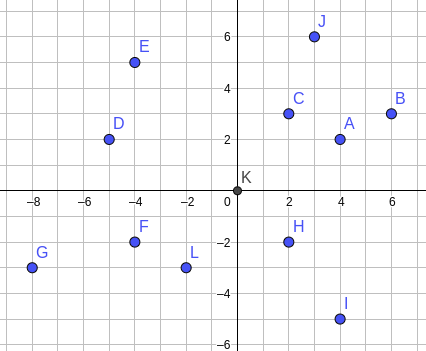
\includegraphics[scale=0.5]{./Images/Transformations/Coords_Ex_1.png}
\end{center}

\begin{exmp}
	Plot the following coordinates one after the other and joining them with a line:

	$(0, 0)$, $(2, 2)$, $(4, 2)$, $(7, 0)$, $(4, -2)$, $(2, -2)$ and $(0,0)$

	Now on the same grid do the same with these points

	$(2, 0)$, $(3, 1)$, $(4, 0)$ and $(3, -1)$

	We should end up with a really bad picture of an eye
	\begin{center}
	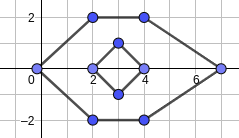
\includegraphics[scale=0.5]{./Images/Transformations/Coord_eg_2.png}
	\end{center}
\end{exmp}

\subsection{Exercise}
Design your own picture with a set of instructions so that a friend can try and recreate your design.
\section{Translations}
A translation is when we move an object so that its position has changed, but nothing else, it will still be the same size and will not have been rotated.

We will describe our translations by saying how far the shape has moved to the right and how far it has moved up.

\begin{exmp}
	Consider the shape ABC below and the translated shape A'B'C'
	\begin{center}
	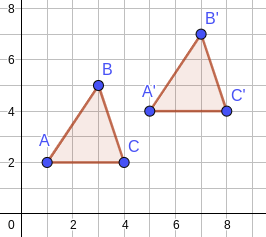
\includegraphics[scale=0.5]{./Images/Transformations/Trans_eg_1.png}
	\end{center}
	Every point has been translated 4 right and 2 up
\end{exmp}

\begin{exmp}
	Consider the shape ABC below and the translated shape A'B'C'
	\begin{center}
	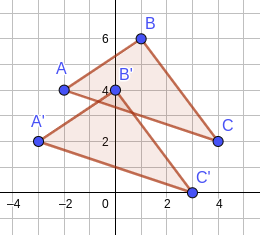
\includegraphics[scale=0.5]{./Images/Transformations/Trans_eg_2.png}
	\end{center}

	Every point has been translated 1 left and 2 down
\end{exmp}

\begin{exmp}
	You can also translate a point
	\begin{center}
	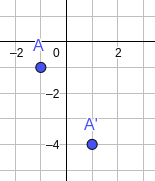
\includegraphics[scale=0.5]{./Images/Transformations/Trans_eg_3.png}
	\end{center}

	The point has been translated 2 right and 3 down
\end{exmp}

\subsection{Exercise}
Describe each of the translations below.  The first one is done for you:

	\begin{center}
		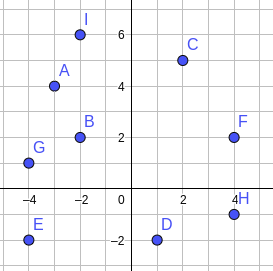
\includegraphics[scale=0.6]{./Images/Transformations/Trans_ex_1.png}
	\end{center}

	\begin{enumerate}
		\item $A \rightarrow B$ right 1, down 2
		\item $A \rightarrow C$ ...
		\item $H \rightarrow D$ ...
		\item $D \rightarrow H$ ...
		\item $E \rightarrow I$ ...
		\item $H \rightarrow E$ ...
		\item $H \rightarrow A$ ...
		\item $B \rightarrow I$ ...
		\item $F \rightarrow F$ ...
		\item $G \rightarrow E$ ...
		\item $D \rightarrow C$ ...
		\item $C \rightarrow G$ ...
	\end{enumerate}

\subsection{Exercise}
	If we had a general point $(x,y)$ and we described its translation as $(x,y) \rightarrow (x+2,y-4)$

	This would mean the translation was 2 right, 4 down.

	Describe the following translations:
	\begin{enumerate}
		\item $(x,y) \rightarrow (x+3,y+5)$
		\item $(x,y) \rightarrow (x-6,y+1)$
		\item $(x,y) \rightarrow (x,y-4)$
		\item $(x,y) \rightarrow (x+4,y)$
	\end{enumerate}

	We can also display a translation with a vector where we show the hoizontal move above the vertical move.
\section{Reflections}
\section{Rotations}
\section{Combinations}
